\documentclass[a4paper]{scrartcl}%{{{

\usepackage{float}
\usepackage{tikz}
\usetikzlibrary{arrows,automata}
\usepackage{pgf}
\usepackage[utf8]{inputenc} % this is needed for umlauts
\usepackage[ngerman]{babel} % this is needed for umlauts
\usepackage[T1]{fontenc}    % this is needed for correct output of umlauts in pd
\usepackage{amssymb}
\usepackage{amsmath}
\usepackage{mathabx}
\usepackage{mathrsfs}
\usepackage{dsfont}
\usepackage{graphicx}
\usepackage{fancyhdr}
\usepackage{lastpage}
\usepackage{imakeidx}
\setlength{\parskip}{\medskipamount}
\setlength{\parindent}{0pt}
\usepackage{enumitem}
\usepackage{hyperref}
\usepackage{verbatim}

%%%%%%%%%%%%%%%%%%%%%%%%
% Kopf- und Fusszeilen %
%%%%%%%%%%%%%%%%%%%%%%%%
\pagestyle{fancy}
\lhead{
        Maximilian Roth
}
\chead{Logik-Tutorat Lösungen Blatt 9\\}
\rhead{
    \begin{tabular}{rr}
        \today{} \\
        Seite \thepage{} von \pageref{LastPage}
    \end{tabular}
}
\lfoot{}
\cfoot{}
\rfoot{} 

%%%%%%%%%%%%%%%%%%%%%%%%
% Anfang des Dokuments %
%%%%%%%%%%%%%%%%%%%%%%%%%}}}

\begin{document}
\section*{Disclaimer}%{{{
\label{sec:disclaimer}
Auch in diesem Dokument können sich Fehler befinden!\\
Sie sind nicht die Musterlösung der Aufgaben, sondern selbst erstellte Lösungen.\\

Als generelle Lektüre kann ich nur das Skript von Markus Junker aus dem WS 17/18 empfehlen:\\
\url{http://home.mathematik.uni-freiburg.de/junker/skripte/InfoLogik.pdf}\\
Hier ist vieles sehr genau und verständlich erklärt.%}}}

\section*{}%{{{
\label{sec:aufgabe_1}

    \begin{figure}[H]
        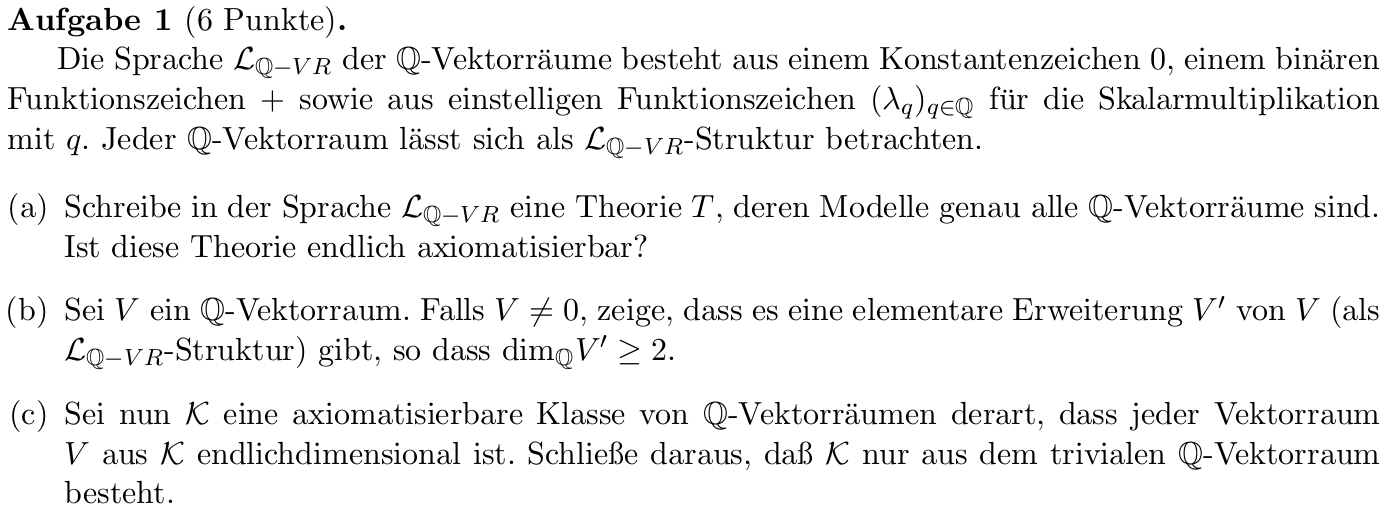
\includegraphics[scale=0.3]{./A-1.png}
        \label{fig:}
    \end{figure}

%}}}

\label{sec:aufgabe_2}%{{{

    \begin{figure}[H]
        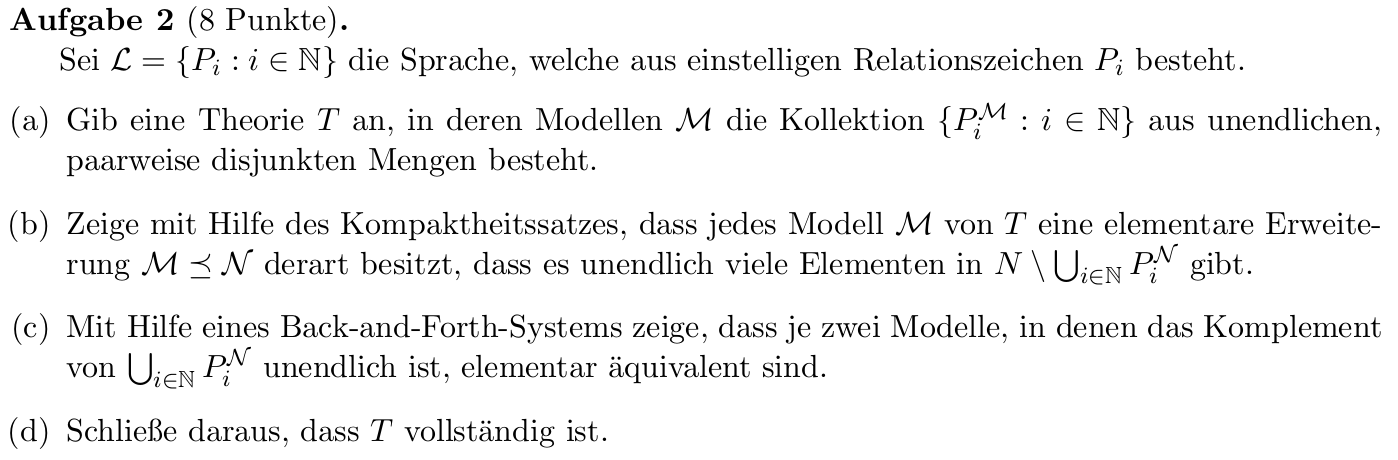
\includegraphics[scale=0.3]{./A-2.png}
        \label{fig:}
    \end{figure}

    \begin{itemize}
        \item a)\\
            Unsere Theorie muss enthalten:\\
            \begin{itemize}
                \item Jedes $P_i^\mathcal{M}$ hat unendlich viele verschiedene Elemente\\
                \item Je zwei $P_i, P_j$ haben kein gleiches Element\\
            \end{itemize}
            Und als Theorie:\\
            $T = \{\exists k_1,\dots,k_n(\bigwedge_{i \neq j} \neg k_i \doteq k_j) \land P_x(k_i)| n,x \in \mathds{N}, i,j\leq n\}\\
            \cup \{\neg \exists x (P_i(x) \land P_j(x)) | i \neq j \in \mathds{N}\}$\\

        \item c)\\
            Wir zeigen, dass es ein nichtleeres Back \& Forth-System mit der Kollektion S gibt.\\
            
            \begin{itemize}
                \item S ist nichtleer\\
                    Seien $\mathcal{M}, \mathcal{N}$ solche Strukturen.\\
                    Wenn gilt $n \in P_i^\mathcal{N} \text{, sowie } m \in P_j^\mathcal{M}$, dann ist $F: \{n\} \rightarrow \{m\}$ partieller Iso.\\
                    Dies geht immer, da die $P_i$ existieren und unendlich groß sein müssen.\\
                    $\Rightarrow$ S ist nichtleer\\
                \item Back \& Forth-System\\
                    \begin{itemize}
                        \item \framebox{Back}\\
                            Sei $F \in S, n \in N\backslash Im(F)$\\
                            \\Wir unterscheiden in: \underline{n ist in einer Menge $P_i$} und \underline{N ist nicht in einer Menge $P_i$}\\
                            \begin{itemize}
                                \item $n \in P_i^\mathcal{N}, i \in \mathds{N}\\
                                    \Rightarrow m \in P_i^\mathcal{M} \backslash Dom(F)$\\
                                \item 
                            \end{itemize}
                            
                    \end{itemize}
            \end{itemize}
    \end{itemize}
%}}}

\section*{}%{{{
\label{sec:aufgabe_3}

    \begin{figure}[H]
        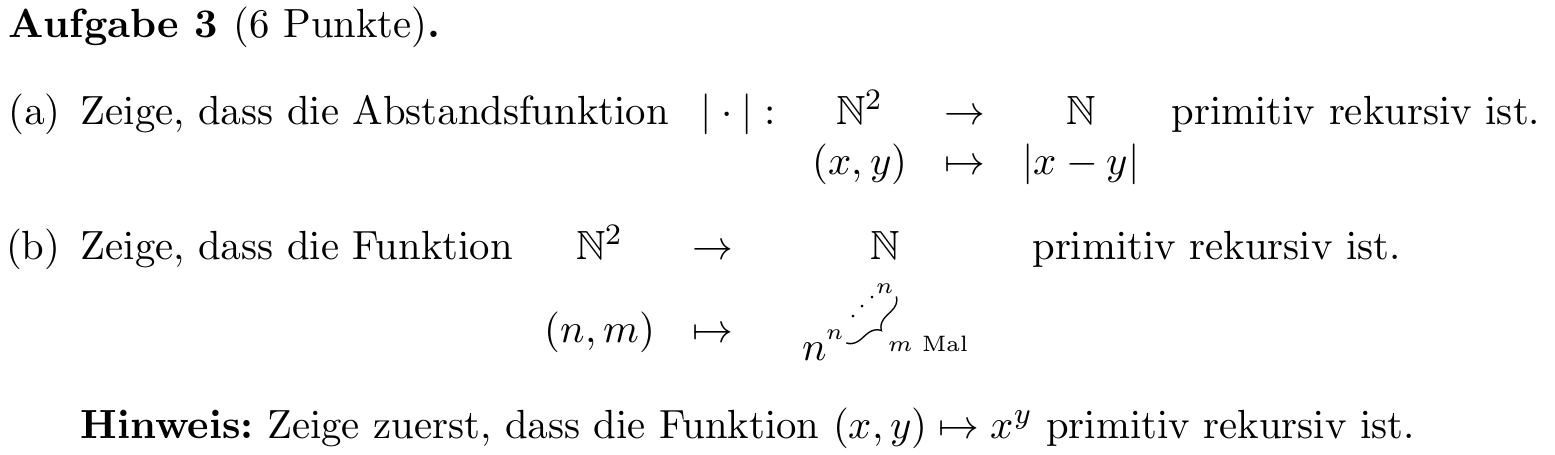
\includegraphics[scale=0.3]{./A-3.png}
        \label{fig:}
    \end{figure}

    \begin{itemize}
        \item a)\\
            $|x-y| := (x \dotdiv y) + (y \dotdiv x)$\\
            Sowohl +, als auch $\dotdiv$ sind p. rek.\\
        \item b)\\
            Wir zeigen $x^y$ p. rek.:\\
            $x^y := \begin{cases}
                        1, &\text{ falls }y=0\\
                        x \cdot x^{y-1}, &\text{ sonst }
                    \end{cases}$\\
            \\Und damit jetzt:\\
            $f(n,m) = \begin{cases}
                n, &\text{ falls }m=0\\
                n^{f(n,m-1)}, &\text{ sonst}
            \end{cases}$\\

    \end{itemize}

    
%}}}

\end{document}

